\chapter[Metodologia]{Metodologia}

	\section[Estrutura Analítica do Projeto - EAP]{Estrutura Analítica do Projeto - EAP}

	\begin{figure}[H]
		\centering
		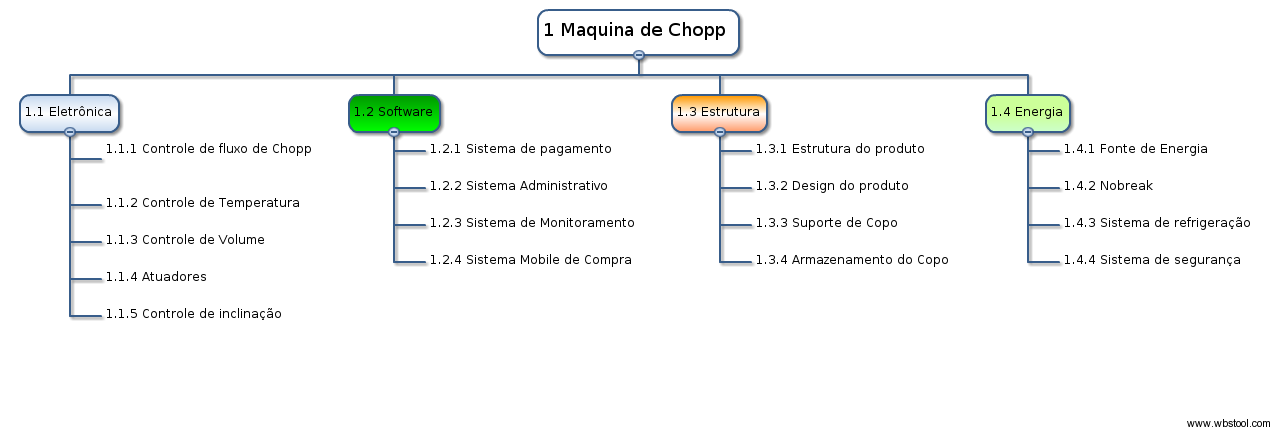
\includegraphics[scale= 0.4]{figuras/eap.png}
		\caption{EAP do projeto.}
		\label{eap}
	\end{figure}

	\section[Tempo]{Tempo}
		Para gerenciar o tempo no projeto, foi usado como base os processos de gerenciamento de tempo baseando-se nas 
		fases de iniciação, planejamento, execução e encerramento, onde cada uma das três grandes entregas do projeto (
		Pontos de Controle 1, 2 e 3) abrangem essas fases. Para o sucesso do mesmo, a equipe precisará cumprir as 
		atividades listadas no cronograma.

		A partir do escopo do projeto, foi feito o cronograma inicial utilizando o software Gantter armazenado no 
		Google Drive para que todos os membros do projeto possam acessá-lo e assim fazer o controle do cronograma, 
		garantindo a transparência e visibilidade a todos para que todos estejam cientes do andamento.

		\subsection[Cronograma]{Cronograma}
			\begin{figure}[H]
				\centering
				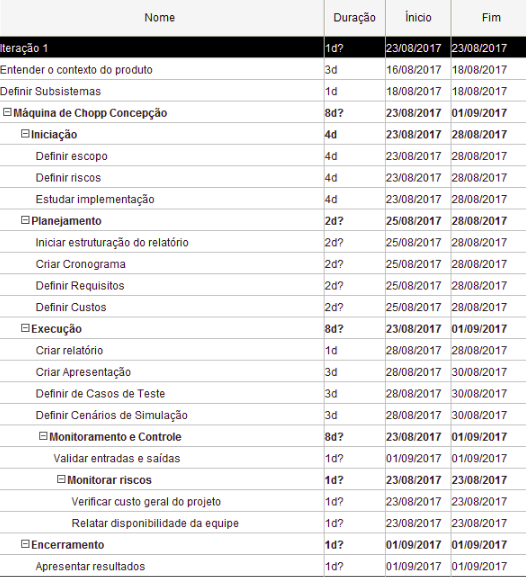
\includegraphics[scale= 0.9]{figuras/cronograma1.png}
				\caption{Cronograma da Primeira Parte do Projeto.}
				\label{cronograma1}
			\end{figure}

			\begin{figure}[H]
				\centering
				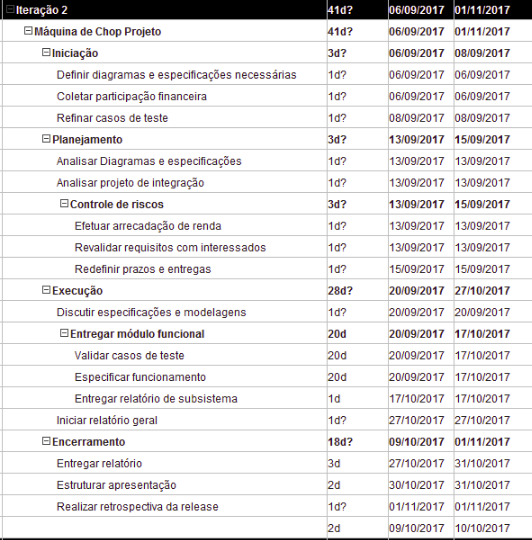
\includegraphics[scale= 0.7]{figuras/cronograma2.png}
				\caption{Cronograma da Segunda Parte do Projeto.}
				\label{cronograma2}
			\end{figure}

			\begin{figure}[H]
				\centering
				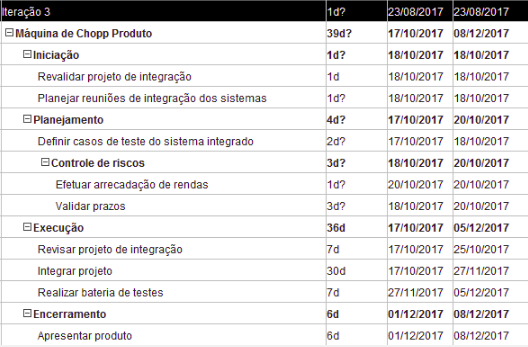
\includegraphics[scale= 0.7]{figuras/cronograma3.png}
				\caption{Cronograma da Terceira Parte do Projeto.}
				\label{cronograma3}
			\end{figure}

	\section[Comunicação]{Comunicação}

		Para uma gestão de excelência de grandes equipes, uma comunicação efetiva é essencial e de extrema importância 
		para evitar maiores preocupações. Esse fator pode ser determinante para o sucesso ou fracasso do projeto, de 
		modo contínuo, desde o planejamento até a integração dos subsistemas. O grupo, na elaboração do projeto 
		Autochopp, utilizou o Slack para comunicação geral dos integrantes, o Google Drive para armazenamento edição 
		colaborativa de arquivos e atividades conjuntas; o Github para o desenvolvimento colaborativo do código e 
		relatório final. Com isso, reuniões periódicas foram feitas com os integrantes do grupo, principalmente para 
		tratar assuntos que precisassem da presença de todos.

